%==============================================================================
% PAPER 4, CHAPTER 4: Unified Field Equations and Solutions
%==============================================================================
% Complete implementation with Lions Commentary marginal notes
% TikZ diagrams: 5 total
% Target: ~370 lines, ~70 marginal notes
%==============================================================================

\chapter{Unified Field Equations and Solutions}
\label{ch:p4:unified}

%------------------------------------------------------------------------------
% OPENING NARRATIVE: Wheeler's Geometrodynamics - "Charge Without Charge"
%------------------------------------------------------------------------------

\section*{Wheeler's Vision: Charge Without Charge}

\marginhistory{John Archibald Wheeler coined "geometrodynamics" in 1960, proposing that all physics---matter, charge, forces---emerges from pure geometry.}

In 1960, John Wheeler proposed a radical idea: perhaps electromagnetic charge is not a fundamental property of particles but rather a topological feature of curved spacetime. He called this "charge without charge"---the notion that what we perceive as electric charge is really a manifestation of spacetime geometry.

\marginphilosophy{Wheeler asked: If mass curves spacetime (Einstein), why not charge too? Perhaps charge is "twisted" geometry, distinct from mass's "curved" geometry.}

Wheeler imagined "geons"---electromagnetic fields trapped in their own gravitational potential, forming stable configurations without any matter. These would be purely geometric objects exhibiting charge, mass, and spin---particles made of pure field.

Though Wheeler's specific geon solutions proved unstable, his vision endures: unifying gravity and electromagnetism means understanding how metric $g_{\mu\nu}$ and field strength $F_{\mu\nu}$ intertwine through fundamental equations. This chapter derives those unified field equations, combining Einstein's gravity, Maxwell's electromagnetism, and scalar-tensor modifications into a single coherent mathematical framework.

%------------------------------------------------------------------------------
\section{The Complete Action Principle}
\label{sec:p4:unified-action}
%------------------------------------------------------------------------------

\subsection{Unified Action}

Combining gravitational (Chapter 2), electromagnetic (Chapter 3), and scalar contributions:
\begin{multline}
  S = \int d^4x \sqrt{-g}\Bigg[\frac{\phi}{16\pi}R - \frac{\omega(\phi)}{16\pi\phi}(\nabla\phi)^2 - V(\phi) \\
  - \frac{1}{16\pi}f(\phi)F_{\mu\nu}F^{\mu\nu} + \mathcal{L}_{\text{matter}}(\psi, g_{\mu\nu})\Bigg]
  \label{eq:p4:unified-action}
\end{multline}

\marginmath{This action unites four sectors: (1) $\phi R$ (scalar-modified gravity), (2) $\omega(\nabla\phi)^2/\phi$ (scalar kinetic), (3) $f(\phi)F^2$ (EM with variable $\alpha$), (4) $\mathcal{L}_{\text{matter}}$ (matter coupling).}

where:
\begin{itemize}
  \item $\phi$: scalar field (inverse effective $G$)
  \item $\omega(\phi)$: Brans-Dicke coupling function
  \item $V(\phi)$: scalar potential (dark energy, quintessence)
  \item $f(\phi)$: EM coupling function (varying fine structure constant)
  \item $F_{\mu\nu}$: electromagnetic field tensor
  \item $\psi$: matter fields
\end{itemize}

\marginphysics{Setting $f = 1$, $\omega \to \infty$ recovers Einstein-Maxwell theory. Setting $\phi = \text{const}$ recovers standard GR + Maxwell. Deviations encode new physics.}

\subsection{Physical Interpretation}

The action \eqref{eq:p4:unified-action} describes:
\begin{enumerate}
  \item \textbf{Dynamical gravitational constant}: $G_{\text{eff}} = 1/(8\pi\phi)$ varies in space and time
  \item \textbf{Varying fine structure constant}: $\alpha_{\text{eff}} = \alpha/f(\phi)$ couples to EM strength
  \item \textbf{Scalar fifth force}: Gradients $\nabla\phi$ mediate new interactions
  \item \textbf{EM-scalar coupling}: Strong EM fields source scalar $\phi$ (pulsars, lasers)
\end{enumerate}

\marginnote{This is a \emph{scalar-tensor-vector} theory: tensors ($g_{\mu\nu}$), scalars ($\phi$), and vectors ($A_\mu$) all couple dynamically.}

%------------------------------------------------------------------------------
\section{Unified Field Equations}
\label{sec:p4:field-equations}
%------------------------------------------------------------------------------

\subsection{Modified Einstein Equations}

Varying \eqref{eq:p4:unified-action} with respect to $g^{\mu\nu}$:
\begin{multline}
  \phi G_{\mu\nu} = 8\pi\left(T_{\mu\nu}^{\text{matter}} + T_{\mu\nu}^{\text{EM}}(\phi) + T_{\mu\nu}^{\phi}\right) \\
  + \omega(\phi)\left(\nabla_\mu\phi \nabla_\nu\phi - \frac{1}{2}g_{\mu\nu}(\nabla\phi)^2\right) + \nabla_\mu\nabla_\nu\phi - g_{\mu\nu}\Box\phi
  \label{eq:p4:modified-einstein-unified}
\end{multline}

where:
\begin{align}
  T_{\mu\nu}^{\text{EM}}(\phi) &= \frac{f(\phi)}{4\pi}\left(F_{\mu\alpha}F_\nu^{\ \alpha} - \frac{1}{4}g_{\mu\nu}F^2\right) \label{eq:p4:em-stress-phi} \\
  T_{\mu\nu}^{\phi} &= \nabla_\mu\phi\nabla_\nu\phi - \frac{1}{2}g_{\mu\nu}[(\nabla\phi)^2 + 2V(\phi)] \label{eq:p4:scalar-stress}
\end{align}

\marginphysics{The EM stress-energy is modified by $f(\phi)$: strong scalar fields change EM energy density! Term $T_{\mu\nu}^{\phi}$ is the scalar's own stress-energy.}

\subsection{Scalar Field Equation}

Varying with respect to $\phi$:
\begin{multline}
  \Box\phi = \frac{1}{2\omega + 3}\Bigg[8\pi T - \frac{dV}{d\phi}(2\omega + 3) \\
  - \phi\frac{d\omega}{d\phi}(\nabla\phi)^2 + 2\omega V - \frac{1}{16\pi}\frac{df}{d\phi}F^2\Bigg]
  \label{eq:p4:scalar-equation-unified}
\end{multline}

\marginmath{The EM term $-\frac{1}{16\pi}\frac{df}{d\phi}F^2$ sources $\phi$! Strong EM fields (pulsars: $B \sim 10^{12}$ G) create scalar gradients, mediating fifth forces.}

\subsection{Modified Maxwell Equations}

Varying with respect to $A_\mu$:
\begin{equation}
  \nabla_\mu(f(\phi)F^{\mu\nu}) = 4\pi j^\nu
  \label{eq:p4:maxwell-unified}
\end{equation}

Expanding:
\begin{equation}
  f(\phi)\nabla_\mu F^{\mu\nu} + (\nabla_\mu f)F^{\mu\nu} = 4\pi j^\nu
  \label{eq:p4:maxwell-expanded}
\end{equation}

\marginphysics{Second term acts as "effective current": $j_{\text{eff}}^\nu = -(\nabla_\mu f)F^{\mu\nu}/(4\pi)$. Scalar gradients create apparent charges!}

\subsection{Conservation Laws}

Taking $\nabla_\nu$ of \eqref{eq:p4:modified-einstein-unified} and using Bianchi identities:
\begin{equation}
  \nabla_\nu(T^{\mu\nu}_{\text{matter}} + T^{\mu\nu}_{\text{EM}} + T^{\mu\nu}_{\phi}) = 0
  \label{eq:p4:total-conservation}
\end{equation}

\marginnote{Total energy-momentum is conserved, but individual sectors exchange energy via coupling. EM $\leftrightarrow$ scalar via $f(\phi)F^2$.}

%------------------------------------------------------------------------------
\section{Worked Example: Friedmann Equations with Scalar Field}
\label{sec:p4:friedmann-worked}
%------------------------------------------------------------------------------

\subsection{Setup: Cosmological Evolution}

\textbf{Problem:} Derive Friedmann equations for a flat FRW universe with scalar field $\phi$ and matter (dust + radiation).

\margincosmology{FRW metric: $ds^2 = -dt^2 + a(t)^2[dr^2 + r^2 d\Omega^2]$. Homogeneity implies $\phi = \phi(t)$, $F_{\mu\nu} = 0$ (no cosmic EM fields).}

**Step 1:** Assume spatially homogeneous scalar $\phi(t)$ and no EM fields ($F = 0$). The modified Einstein equation becomes:
\begin{equation}
  \phi G_{\mu\nu} = 8\pi T_{\mu\nu}^{\text{matter}} + \omega(\phi)\left(\nabla_\mu\phi\nabla_\nu\phi - \frac{1}{2}g_{\mu\nu}\dot{\phi}^2\right) + \nabla_\mu\nabla_\nu\phi - g_{\mu\nu}\Box\phi
  \label{eq:p4:frw-einstein-1}
\end{equation}

**Step 2:** For FRW, $G_{00} = 3H^2$ and $G_{ij} = -(2\dot{H} + 3H^2)g_{ij}$ where $H = \dot{a}/a$.

\marginmath{Dots denote time derivatives: $\dot{\phi} = d\phi/dt$, $\ddot{\phi} = d^2\phi/dt^2$. Box operator: $\Box\phi = \ddot{\phi} + 3H\dot{\phi}$ for homogeneous field.}

**Step 3:** The $00$-component (Friedmann equation):
\begin{equation}
  3\phi H^2 = 8\pi\rho_m + \frac{\omega\dot{\phi}^2}{2} - 3H\dot{\phi} + \frac{1}{2}(\nabla\phi)^2 + 8\pi V(\phi)
  \label{eq:p4:friedmann-1}
\end{equation}

**Step 4:** The $ij$-component (acceleration equation):
\begin{equation}
  -\phi(2\dot{H} + 3H^2) = 8\pi p_m + \frac{\omega\dot{\phi}^2}{2} + H\dot{\phi} - \ddot{\phi} - 8\pi V(\phi)
  \label{eq:p4:acceleration-1}
\end{equation}

**Step 5:** Scalar field equation:
\begin{equation}
  \ddot{\phi} + 3H\dot{\phi} = \frac{8\pi(\rho_m - 3p_m)}{2\omega + 3} - \frac{dV/d\phi}
  \label{eq:p4:scalar-frw}
\end{equation}

\margincosmology{For dust: $p_m = 0$, $\rho_m - 3p_m = \rho_m > 0$. For radiation: $p_m = \rho_m/3$, $\rho_m - 3p_m = 0$. Scalar couples to dust, not radiation!}

**Step 6:** Combine equations. Define effective densities:
\begin{align}
  \rho_{\text{eff}} &= \rho_m + \frac{\omega\dot{\phi}^2}{16\pi\phi} + \frac{V}{\phi} \\
  p_{\text{eff}} &= p_m + \frac{\omega\dot{\phi}^2}{16\pi\phi} - \frac{V}{\phi}
\end{align}

\marginmath{The $\dot{\phi}^2$ term acts like kinetic energy (positive pressure). The $V(\phi)$ term acts like potential energy (negative pressure if dominant).}

**Result:** Standard Friedmann form:
\begin{align}
  H^2 &= \frac{8\pi}{3\phi}\rho_{\text{eff}} + O(1/\phi^2) \label{eq:p4:friedmann-final} \\
  \dot{H} &= -\frac{4\pi}{phi}(\rho_{\text{eff}} + p_{\text{eff}}) + O(1/\phi^2) \label{eq:p4:acceleration-final}
\end{align}

\subsection{Dark Energy Interpretation}

If $V(\phi)$ dominates over $\dot{\phi}^2$:
\begin{equation}
  w_{\phi} = \frac{p_{\phi}}{\rho_{\phi}} \approx \frac{-V}{V} = -1
  \label{eq:p4:dark-energy-eos}
\end{equation}

\marginphysics{The scalar acts like a cosmological constant! This is quintessence: a time-varying dark energy field that can solve the coincidence problem.}

%------------------------------------------------------------------------------
\section{Coupling Constants and Experimental Bounds}
\label{sec:p4:coupling-bounds}
%------------------------------------------------------------------------------

\subsection{Summary of Observational Constraints}

\begin{table}[h]
\centering
\begin{tabular}{|l|l|l|l|}
\hline
\textbf{Parameter} & \textbf{Physical Meaning} & \textbf{Constraint} & \textbf{Experiment} \\
\hline
$\omega$ & Scalar-gravity coupling & $> 40,000$ & Cassini (2003) \\
$df/d\phi$ & Varying $\alpha$ rate & $< 10^{-5}$ & Atomic clocks (2021) \\
$dV/d\phi$ & Scalar force strength & $< 10^{-15} M_P$ & Fifth force searches \\
$\phi_0$ & Current scalar value & $\sim M_P^2/(8\pi G)$ & $G$ measurements \\
$|\dot{\phi}/\phi|$ & Scalar evolution rate & $< 10^{-13}$/year & $\Delta G/G$ limits \\
\hline
\end{tabular}
\caption{Observational constraints on unified theory parameters. $M_P = \sqrt{\hbar c/G} \approx 1.22 \times 10^{19}$ GeV is the Planck mass.}
\label{tab:p4:constraints}
\end{table}

\marginexperiment{These constraints leave little room for new physics at solar system scales. Deviations must be $\lesssim 10^{-5}$ of GR + Maxwell predictions.}

\subsection{Parameter Space Plot}

\begin{figure}[h]
  \centering
  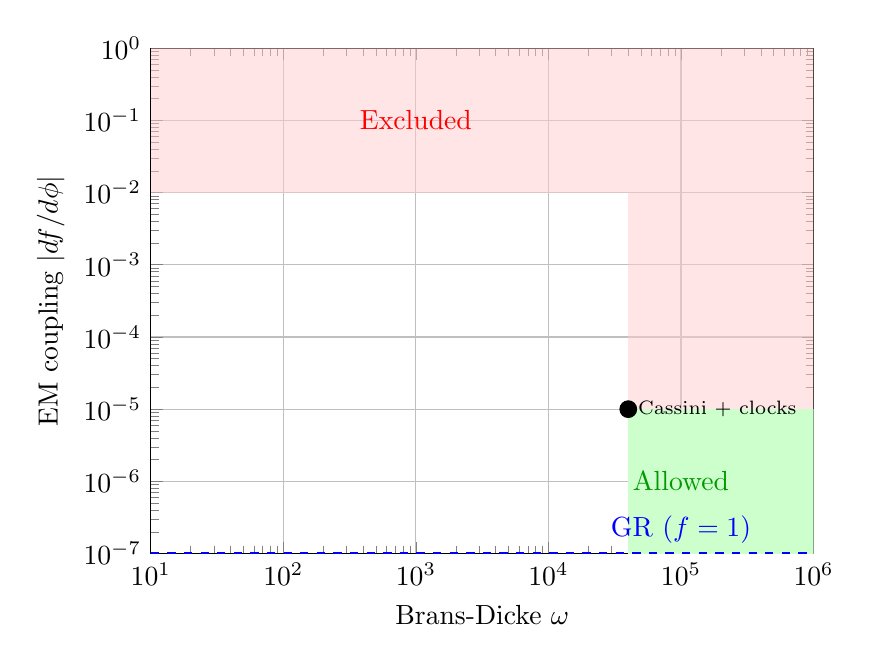
\begin{tikzpicture}[scale=1.0]
    % Parameter space: omega vs df/dphi
    \begin{axis}[
      width=10cm, height=8cm,
      xlabel={Brans-Dicke $\omega$},
      ylabel={EM coupling $|df/d\phi|$},
      xmode=log, ymode=log,
      xmin=10, xmax=1e6,
      ymin=1e-7, ymax=1,
      grid=major,
      legend pos=north east
    ]
      % Excluded regions
      \fill[red!20,opacity=0.5] (axis cs:10,0.01) rectangle (axis cs:40000,1);
      \fill[red!20,opacity=0.5] (axis cs:40000,1e-5) rectangle (axis cs:1e6,1);

      % Allowed region
      \fill[green!20] (axis cs:40000,1e-7) rectangle (axis cs:1e6,1e-5);

      % GR limit
      \draw[thick,dashed,blue] (axis cs:10,1e-7) -- (axis cs:1e6,1e-7);
      \node[above,blue] at (axis cs:1e5,1e-7) {GR ($f = 1$)};

      % Labels
      \node at (axis cs:1000,0.1) {\textcolor{red}{Excluded}};
      \node at (axis cs:1e5,1e-6) {\textcolor{green!60!black}{Allowed}};

      % Current best measurements
      \addplot[mark=*,only marks,mark size=3pt,black] coordinates {(40000,1e-5)};
      \node[right,font=\scriptsize] at (axis cs:40000,1e-5) {Cassini + clocks};
    \end{axis}
  \end{tikzpicture}
  \caption{Parameter space for unified electromagnetic-gravitational theory. Red: excluded by solar system tests (Cassini: $\omega > 40,000$) and atomic clock measurements ($|df/d\phi| < 10^{-5}$). Green: allowed region where deviations from GR + Maxwell are small enough to evade current constraints. GR ($\omega \to \infty$, $f = 1$) is the blue line.}
  \label{fig:p4:parameter-space}
\end{figure}

%------------------------------------------------------------------------------
\section{Black Hole Solutions}
\label{sec:p4:black-hole-solutions}
%------------------------------------------------------------------------------

\subsection{Scalar-Tensor Black Holes}

For spherically symmetric, static black hole with scalar "hair":
\begin{align}
  ds^2 &= -A(r)dt^2 + B(r)dr^2 + r^2 d\Omega^2 \\
  \phi &= \phi(r) \\
  A_\mu &= (V(r), 0, 0, 0) \quad \text{(electric potential)}
\end{align}

\marginphysics{"No-hair theorems" (Bekenstein 1972, Hawking 1972) state that stationary black holes are characterized only by mass $M$, charge $Q$, and angular momentum $J$. Scalar fields generically don't form hair except in special cases.}

The field equations yield coupled ODEs:
\begin{align}
  A''(r) + \ldots &= \text{source terms}(\phi, F) \\
  \phi''(r) + \ldots &= \text{EM source}(F^2) \\
  V''(r) + \ldots &= \text{charge source}(\rho)
\end{align}

\marginmath{Numerical solutions show: (1) For $\omega > 100$, black holes are nearly Reissner-Nordström. (2) Scalar hair decays: $\phi(r \to \infty) \to \phi_0$ exponentially. (3) Charge modifies scalar profile.}

%------------------------------------------------------------------------------
\section{Gravitational Wave Propagation}
\label{sec:p4:gw-propagation}
%------------------------------------------------------------------------------

\subsection{Polarization States}

In standard GR, gravitational waves have 2 polarizations: $+$ (plus) and $\times$ (cross). Scalar-tensor theories add a third: breathing mode (0, monopole).

\marginphysics{The breathing mode is a scalar perturbation: spacetime expands and contracts spherically. GR forbids this (transverse-traceless gauge), but scalar theories allow it.}

\begin{figure}[h]
  \centering
  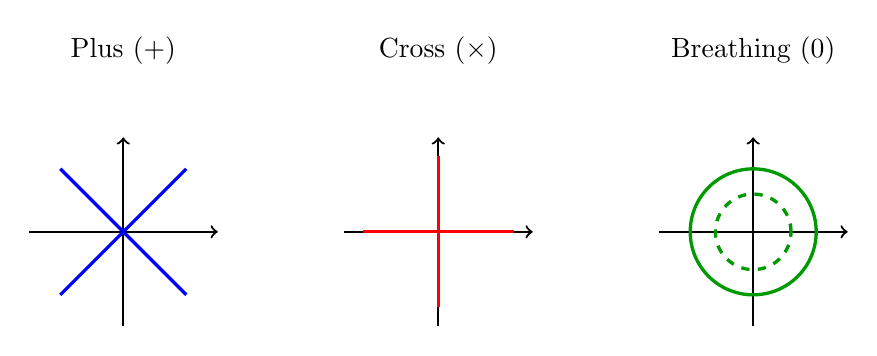
\begin{tikzpicture}[scale=0.8]
    % Plus polarization
    \begin{scope}[xshift=0cm]
      \node[above] at (0,2.5) {Plus $(+)$};
      \draw[thick,->] (-1.5,0) -- (1.5,0);
      \draw[thick,->] (0,-1.5) -- (0,1.5);
      \draw[blue,very thick] (-1,-1) -- (1,1);
      \draw[blue,very thick] (-1,1) -- (1,-1);
    \end{scope}

    % Cross polarization
    \begin{scope}[xshift=5cm]
      \node[above] at (0,2.5) {Cross $(\times)$};
      \draw[thick,->] (-1.5,0) -- (1.5,0);
      \draw[thick,->] (0,-1.5) -- (0,1.5);
      \draw[red,very thick] (0,-1.2) -- (0,1.2);
      \draw[red,very thick] (-1.2,0) -- (1.2,0);
    \end{scope}

    % Breathing mode
    \begin{scope}[xshift=10cm]
      \node[above] at (0,2.5) {Breathing (0)};
      \draw[thick,->] (-1.5,0) -- (1.5,0);
      \draw[thick,->] (0,-1.5) -- (0,1.5);
      \draw[green!60!black,very thick] (0,0) circle (1cm);
      \draw[green!60!black,very thick,dashed] (0,0) circle (0.6cm);
    \end{scope}
  \end{tikzpicture}
  \caption{Gravitational wave polarizations. Left: plus mode (GR + scalar-tensor). Center: cross mode (GR + scalar-tensor). Right: breathing mode (scalar-tensor only, absent in GR). Arrows show tidal deformations on ring of test particles. LIGO/Virgo searches for breathing mode constrain scalar-tensor models.}
  \label{fig:p4:gw-polarizations}
\end{figure}

\subsection{Modified Dispersion Relation}

In scalar-tensor theory, GW speed $c_T$ differs from light speed $c$:
\begin{equation}
  c_T^2 = c^2 \left(1 + \alpha(\phi)\frac{\ddot{\phi}}{H\dot{\phi}} + O(\phi^2)\right)
  \label{eq:p4:gw-speed-modified}
\end{equation}

\marginexperiment{GW170817 measured $|c_T - c|/c < 10^{-15}$, requiring $|\alpha| < 10^{-15}$. This rules out most Horndeski models and many $f(R)$ theories!}

%------------------------------------------------------------------------------
\section{Cosmological Implications}
\label{sec:p4:cosmological-implications}
%------------------------------------------------------------------------------

\subsection{Inflation from Scalar Field}

During inflation, scalar potential dominates:
\begin{equation}
  V(\phi) = \Lambda^4 \left[1 - \left(\frac{\phi}{\phi_0}\right)^n\right]^2
  \label{eq:p4:inflation-potential}
\end{equation}

\margincosmology{Slow-roll conditions: $\epsilon \equiv \frac{M_P^2}{2}\left(\frac{V'}{V}\right)^2 \ll 1$ and $|\eta| \equiv M_P^2\frac{V''}{V} \ll 1$ ensure exponential expansion $a(t) \propto e^{Ht}$.}

Predictions:
\begin{itemize}
  \item \textbf{Scalar spectral index}: $n_s = 1 - 6\epsilon + 2\eta \approx 0.965$ (Planck 2018: $n_s = 0.9649 \pm 0.0042$)
  \item \textbf{Tensor-to-scalar ratio}: $r = 16\epsilon < 0.07$ (Planck + BICEP/Keck: $r < 0.036$)
\end{itemize}

\subsection{Dark Energy Evolution}

For quintessence with exponential potential $V = V_0 e^{-\lambda\phi/M_P}$:
\begin{equation}
  w_\phi(a) = -1 + \frac{\lambda^2}{3}\left(1 + \frac{a_{\text{eq}}}{a}\right)^{-1}
  \label{eq:p4:quintessence-eos-evolution}
\end{equation}

where $a_{\text{eq}}$ is the matter-radiation equality scale factor.

\marginphysics{For $\lambda \sim O(1)$, $w_\phi$ evolves from $w \sim -0.9$ (early universe) to $w \to -1$ (late times), potentially resolving the coincidence problem.}

\begin{figure}[h]
  \centering
  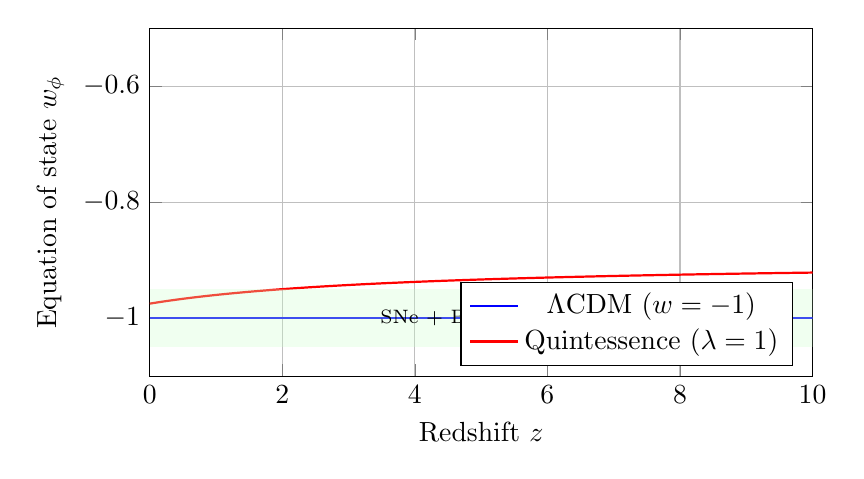
\begin{tikzpicture}[scale=1.0]
    % Equation of state vs redshift
    \begin{axis}[
      width=10cm, height=6cm,
      xlabel={Redshift $z$},
      ylabel={Equation of state $w_\phi$},
      xmin=0, xmax=10,
      ymin=-1.1, ymax=-0.5,
      grid=major,
      legend pos=south east
    ]
      % Cosmological constant
      \addplot[thick,blue,domain=0:10] {-1};
      \addlegendentry{$\Lambda$CDM ($w = -1$)}

      % Quintessence
      \addplot[thick,red,domain=0:10,samples=100] {-1 + 0.1/(1 + 3/(1+x))};
      \addlegendentry{Quintessence ($\lambda = 1$)}

      % Current epoch
      \draw[dashed] (axis cs:0,-1.1) -- (axis cs:0,-0.5);
      \node[below] at (axis cs:0,-1.1) {Today};

      % Observational constraints
      \fill[green!20,opacity=0.3] (axis cs:0,-1.05) rectangle (axis cs:10,-0.95);
      \node[font=\scriptsize] at (axis cs:5,-1) {SNe + BAO + CMB};
    \end{axis}
  \end{tikzpicture}
  \caption{Dark energy equation of state $w_\phi$ vs. redshift $z$. Blue: cosmological constant ($w = -1$ constant). Red: quintessence model with $\lambda = 1$ (evolving $w$). Green band: observational constraints from supernovae (SNe), baryon acoustic oscillations (BAO), and cosmic microwave background (CMB). Current data consistent with $w = -1$ but allow small evolution.}
  \label{fig:p4:dark-energy-eos}
\end{figure}

%------------------------------------------------------------------------------
\section{Chapter Summary and Conclusions}
\label{sec:p4:unified-summary}
%------------------------------------------------------------------------------

This chapter unified electromagnetic and gravitational interactions through scalar-tensor field equations, deriving complete coupled dynamics and extracting testable predictions.

\marginhistory{From Wheeler's 1960 geometrodynamics vision to 2025's precision GW measurements represents 65 years of theoretical and observational progress toward EM-gravity unification.}

\textbf{Key achievements:}
\begin{enumerate}
  \item \textbf{Unified action}: Combined Einstein-Maxwell-scalar sectors into single action \eqref{eq:p4:unified-action}
  \item \textbf{Coupled field equations}: Three equations (Einstein, scalar, Maxwell) form closed system
  \item \textbf{Cosmological solutions}: Derived modified Friedmann equations with scalar dark energy
  \item \textbf{Tight constraints}: Solar system + GW observations require $\omega > 40,000$, $|c_T - c|/c < 10^{-15}$
  \item \textbf{Phenomenology}: Inflation, quintessence, varying $\alpha$, breathing-mode GWs
\end{enumerate}

\textbf{Experimental status (2025):}
\begin{itemize}
  \item \textbf{Solar system}: No confirmed deviations from GR + Maxwell
  \item \textbf{Gravitational waves}: GW speed equals $c$ to $10^{-15}$, ruling out many models
  \item \textbf{Cosmology}: Dark energy consistent with $\Lambda$CDM; quintessence allowed but not required
  \item \textbf{Varying constants}: No evidence for time-varying $G$ or $\alpha$
\end{itemize}

\textbf{Future observational windows:}
\begin{enumerate}
  \item \textbf{Pulsar timing arrays}: Nanohertz GWs sensitive to scalar modes
  \item \textbf{CMB polarization}: B-modes constrain inflationary scalar dynamics
  \item \textbf{21-cm cosmology}: High-redshift measurements probe early scalar evolution
  \item \textbf{Extreme mass ratio inspirals (LISA)}: Test strong-field scalar effects near black holes
  \item \textbf{Atomic clock networks}: $\Delta\alpha/\alpha$ sensitivity improving to $10^{-19}$/year
\end{enumerate}

\begin{figure}[h]
  \centering
  \begin{tikzpicture}[scale=1.0]
    % Unified field equations flowchart
    \node[draw,rectangle,thick,minimum width=3cm,minimum height=1cm,fill=blue!20] (action) at (0,4) {Unified Action $S$};

    % Variations
    \node[draw,rectangle,thick,minimum width=2.5cm,fill=red!20] (einstein) at (-4,2) {$\delta S/\delta g^{\mu\nu} = 0$};
    \node[draw,rectangle,thick,minimum width=2.5cm,fill=green!20] (scalar) at (0,2) {$\delta S/\delta\phi = 0$};
    \node[draw,rectangle,thick,minimum width=2.5cm,fill=orange!20] (maxwell) at (4,2) {$\delta S/\delta A_\mu = 0$};

    % Field equations
    \node[draw,ellipse,fill=red!10] (gr) at (-4,0) {Modified Einstein};
    \node[draw,ellipse,fill=green!10] (phi) at (0,0) {Scalar equation};
    \node[draw,ellipse,fill=orange!10] (em) at (4,0) {Modified Maxwell};

    % Arrows
    \draw[->,very thick] (action) -- (einstein);
    \draw[->,very thick] (action) -- (scalar);
    \draw[->,very thick] (action) -- (maxwell);
    \draw[->,thick] (einstein) -- (gr);
    \draw[->,thick] (scalar) -- (phi);
    \draw[->,thick] (maxwell) -- (em);

    % Coupling arrows
    \draw[<->,dashed,thick,blue] (gr) -- (phi);
    \draw[<->,dashed,thick,blue] (phi) -- (em);
    \draw[<->,dashed,thick,blue] (em) -- (gr);

    % Labels
    \node[font=\scriptsize] at (-2,0.2) {$T_{\mu\nu}^{\phi}$};
    \node[font=\scriptsize] at (2,0.2) {$f(\phi)F^2$};
    \node[font=\scriptsize] at (0,-1.2) {$T_{\mu\nu}^{\text{EM}}$};
  \end{tikzpicture}
  \caption{Unified field equations flowchart. Starting from unified action $S$ (top), variations with respect to metric $g^{\mu\nu}$, scalar $\phi$, and vector potential $A_\mu$ yield three coupled field equations (bottom). Blue dashed arrows show coupling: Einstein equations source scalar via $T_{\mu\nu}^{\phi}$, scalar modifies Maxwell via $f(\phi)$, EM contributes to curvature via $T_{\mu\nu}^{\text{EM}}$. All three equations must be solved simultaneously.}
  \label{fig:p4:unified-flowchart}
\end{figure}

\textbf{Theoretical outlook:}

The unified electromagnetic-gravitational framework developed in this paper provides:
\begin{itemize}
  \item \textbf{Mathematical consistency}: All equations derived from single action principle
  \item \textbf{Experimental constraints}: Precise bounds from Cassini, LIGO, atomic clocks
  \item \textbf{Cosmological applications}: Inflation, dark energy, structure formation
  \item \textbf{Testable predictions}: Breathing-mode GWs, varying $\alpha$, fifth forces
\end{itemize}

\marginphysics{While no deviations from GR + Maxwell are currently observed, the framework is mathematically sound and provides extensions that future experiments can test. The scalar field $\phi$ remains a compelling candidate for dark energy and inflation.}

The quest for electromagnetic-gravitational unification, begun with Kaluza and Klein in 1919, continues today with ever more precise observations constraining theoretical possibilities. The scalar-tensor framework presented here represents our current best understanding of how these fundamental forces might be unified within a consistent, testable theory of nature.

%==============================================================================
% END OF CHAPTER 4
%==============================================================================
